%%%%%%%%%%%%%%%%%%%%%%%%%%%%%%%%%%%%%%%%%%%%%%%%%%%%%%%%%%%%%%%%%%%%%%%%%%%%%
%% 
%% Informal notes on k-randomization.
%% 
%%%%%%%%%%%%%%%%%%%%%%%%%%%%%%%%%%%%%%%%%%%%%%%%%%%%%%%%%%%%%%%%%%%%%%%%%%%%%


\documentclass[11pt]{article}
%\documentclass[11pt,draft]{amsart}

% Custom styling.
\usepackage{custom}
%% Controls enumeration labels
%\usepackage{enumerate}
%% Shrinks margins 
\usepackage{fullpage}
%% Shows equation label keys
%\usepackage[notref]{showkeys}

%% Some shortcuts.
\newcommand{\Dsp}{\mathcal{D}}
\newcommand{\Ssp}{\mathcal{S}}
\newcommand{\zv}{\textbf{0}}
\newcommand{\uv}{\textbf{1}}

%% Title matter
\title{Sufficient Differential Privacy}
\author{Maxim Zhilyaev \and David Zeber}

\usepackage[english]{babel}
\usepackage{graphicx}

%%%%%%%%%%%%%%%%%%%%%%%%%%%%%%%%%%%%%%%%%%%%%%%%%%%%%%%%%%%%%%%%%%%%%%%%%%%%%

\begin{document}
\maketitle


\section{Introduction}

Differential Privacy (DP) is a now standard technique for data reporting with built-in privacy protections that allow for a quantification of the privacy risk taken on by the individuals represented in the dataset.
Although originally geared towards computing aggregate summaries from a database, in recent developments it has been applied to collecting technical data from users of an app or service.

\subsection{Theoretical setting}

The theoretical setting for DP is as follows.
We consider a dataset or collection $D$ consisting of the original, unprotected data. It can be thought of as a vector $D = (x_1,\dots, x_N)$ containing a datapoint $x_i$ for each user $i = 1,\dots,N$, where the $x_i$ are themselves vectors in some arbitrary space $\Dsp$, representing the data collected for each user.
The data are ``reported'' by a mechanism $\map{A}{\Dsp^N}{\Ssp}$ which applies a transformation to the original dataset $D$. For example, $A$ may compute an aggregate statistic, or it may simply report a transformed version of $x_i$ for each user in the collection.
The transformation $A$ is assumed to be randomized, in the sense that the outcome $A(D)$ is a random element of $\Ssp$. This is typically done by injecting random noise in the process of computing $A(D)$.

The privacy guaranteed offered by DP limits how much the outcome of applying $A$ can change when a single user's record is modified, which in turn limits how easily an individual's data value can be determined based on the outcome $A(D)$. 
We represent this modification by a collection $D_m$ formed by modifying the data for exactly one user: $D_m = (x_1,\dots,x_{r-1},x'_r,x_{r+1},\dots,x_N)$ for some $r \in \{1,\dots,N\}$.
The randomized data collection mechanism $A$ satisfies $\epsilon$-\textbf{differential privacy} if
\begin{equation} \label{eq:dpdeftraditional}
\P[A(D_m) \in B] \leq e^\epsilon \cdot\P[A(D) \in B]
\end{equation}
for all $B \cont \Ssp$ given any original dataset $D$ and modified version $D_m$.
If the outcome space $\Ssp$ is finite (discrete), the condition \eqref{eq:dpdeftraditional} can be restricted to single outcomes:
\begin{equation} \label{eq:dpdeftraddiscrete}
\P[A(D_m) = s] \leq e^\epsilon \cdot\P[A(D) = s]
\end{equation}
for all $s\in\Ssp$.

An important subclass of DP algorithms, known as the \textbf{local DP model}, applies randomization independently to each data value $x_i$.
This is useful in situations where each user reports data separately to a common data collector (\eg the app developer) and wants privacy protection to be applied before the data leaves their local device.
In this case,
\begin{equation} \label{eq:localdpmodel}
A(D) = \big(A_0(x_1),\dots,A_0(x_N)\big),
\end{equation}
where $\map{A_0}{\Dsp}{\Dsp}$ is a randomized transformation to be applied to each data element independently.
We refer to the outcome $S = A(D) \in\Dsp^N$ as a synthetic collection.
Because of independence, \eqref{eq:dpdeftraddiscrete} reduces to comparing outcomes only for the element that gets modified:
\begin{equation} \label{eq:dpdeflocal}
\P[A_0(x'_r) = s] \leq e^\epsilon \cdot\P[A_0(x_r) = s].
\end{equation}

Consider rephrasing \eqref{eq:dpdeftraddiscrete} in terms of a ratio of probabilities:
\begin{equation} \label{eq:dpdefratio}
\frac{\P[A(D_m) = S]}{\P[A(D) = S]} \leq e^\epsilon.
\end{equation}
In what follows, we will work with data encoded as bit vectors ($\Dsp = \{0,1\}^L$), and so we maintain the simplifying assumptions that $\Ssp = \Dsp^N$ is finite, and that $\P[A_0(x) = s] > 0$ for any $x, s\in\Dsp$.
We term the ratio in \eqref{eq:dpdefratio} the \textbf{privacy ratio}, and view it as a function of the original, modified and synthetic collections:
\begin{equation*}
R(S;\,D,D_m) = \frac{\P[A(D_m) = S]}{\P[A(D) = S]}.
\end{equation*}
From \eqref{eq:dpdefratio}, $\epsilon$-differential privacy requires that
\[ \max_{D, D_m, S\in\Dsp^N} R(S;\,D,D_m) \leq e^\epsilon. \]
As above, in the local DP case, we have
\begin{equation*}
R(S;\,D,D_m) = R(s;\,x,x') = \frac{\P[A_0(x') = s]}{\P[A_0(x) = s]},
\end{equation*}
and the DP guarantee translates to
\begin{equation*}
\max_{x, x', s\in\Dsp} R(s;\,x,x') \leq e^\epsilon,
\end{equation*}
elementwise over $\Dsp$.

\subsection{Sufficient differential privacy}

Under local DP \eqref{eq:localdpmodel}, we are implicitly assuming that the collections are indexed by user.
For example, there may be a user ID associated with each element of the dataset.
This is encoded in our representation of $D$ and $S$ as vectors with a specific ordering.
Thus, a synthetic dataset where user A reports 1 and user B reports 0 is distinct from one where user A reports 0 and user B reports 1.

%Recall that, in the traditional differential privacy (DP) setting, we take the original dataset $D$ and transform it into a synthetic version $S$, as a part of which the data is subject to randomization.
%The privacy protection guaranteed by a randomized data collection algorithm $A$, which generates the synthetic dataset as $S = A(D)$, is controlled by the \textbf{privacy ratio} $R$. This ratio compares the outcomes for the original dataset $D$ against those for a modified version $D_m$ which is identical to $D$ except for one element which has been modified. 
%More specifically, the privacy ratio can be thought of as a function over the space (discrete in our setting) of all possible synthetic collections $S$:
%\begin{equation} \label{eq:basicpr}
%R(S;\, D, D_m) = \frac{\P[A(D_m) = S]}{\P[A(D) = S]}.
%\end{equation}
%The algorithm $A$ guarantees differential privacy provided 
%\begin{equation}\label{eq:dpdef}
%\log R(S;\,D, D_m) \leq \epsilon
%\end{equation}
%over all synthetic datasets $S$, for any original dataset $D$ and modification $D_m$. 
%In the case of local DP, where randomization is applied independently to each element of the dataset, $R$ depends only on the element that differs between $D$ and $D_m$ and its synthetic version:
%\begin{equation} \label{eq:localpr}
%R(S;\, D, D_m) = R(s;\, x, x_m) = \frac{\P[A(x_m) = s]}{\P[A(x) = s]}.
%\end{equation}
%Note that \eqref{eq:localpr} follows because the synthetic dataset is allowed to retain the ordering of the original, 

Now, suppose that the synthetic data reported under the local model is \textbf{perfectly anonymized}: there is no way to link a record back to the user that reported it, or even to connect records reported by the same user.
In this case, from the point of view of the data collector, synthetic datasets that differ only in ordering are now indistinguishable.
Such a dataset can be thought of as a bag of values rather than an ordered list, and is equivalently represented as a histogram of frequency counts over $\Dsp$.
Intuitively, this setting offers a stronger privacy protection that should scale with the population: a dataset with an unusual true reported value is indistinguishable from one with the same value resulting from the randomization, and obtaining such values by chance should become more likely as the population size grows---it becomes easier to ``hide in the crowd''.

Formally speaking, the $\epsilon$ level in the privacy guarantee (the maximal value of the privacy ratio) remains the same, since the maximal $D$, $D_m$, and $S$ can be passed into \eqref{eq:dpdefratio} regardless of whether the dataset is anonymized.
%However, consider the important special case of bit vectors (elements of the space $\{0, 1\}^L$).
However, under the assumption of perfect anonymization, \eqref{eq:localdpmodel} no longer fully specifies the data reporting mechanism. We can without loss of generality consider $A$ to include a final aggregation step that tallies the synthetic dataset into counts of unique values, as a consequence of which \eqref{eq:dpdeflocal} no longer applies.
In this case, obtaining a synthetic output $S$ from an ``extreme'' $D_m$ that attains the bound \eqref{eq:dpdefratio} becomes less and less likely as the population grows.
Not only this, but the maximal value of $R$ over a subset of the most likely synthetic outcomes is significantly lower.

To take advantage of these consequences of perfect anonymization, we propose an alternative privacy criterion, \textbf{sufficient differential privacy}, under which the privacy condition \eqref{eq:dpdefratio} is allowed to fail with a small probability.
There are two main benefits arising from this approach.
First, it has the potential to drastically reduce the individual randomization noise required to obtain similar privacy levels to local DP, thus greatly improving the utility of the collected data relative to a method like RAPPOR.
Additionally, while the size of the dataset does not play a role in traditional local DP (\ie there is no privacy benefit to having a larger dataset), the privacy and associated noise level become related to the dataset size under sufficient DP, in that a larger dataset requires smaller randomization noise to achieve results of comparable quality.

Given original and modified datasets $D$ and $D_m$, we consider $R(S)$ a random variable: it is the value of the function $R$ for the synthetic dataset which is the random outcome of applying the algorithm $A$ to $D_m$, \ie $S = A(D_m)$.
Its distribution is given by
\begin{equation} \label{eq:prdistrib}
\P\big[R(S;\, D, D_m) \in \cdot\,\big] = \P\big[A(D_m) \in \{S : R(S;\, D, D_m) \in \cdot\,\}\big].
\end{equation}
We say the randomized mechanism $A$ satisfies $(\epsilon, \eta)$-\textbf{sufficient differential privacy} if
\begin{equation}\label{eq:suffpr}
\P[R(S;\, D, D_m) > e^\epsilon] \leq \eta
\end{equation}
for all $D$, $D_m$, and we refer to $\eta$ as the \textbf{probability cut-off}.
Intuitively, we are thinking of $D_m$ as an ``extreme'' dataset where the modified element carries a high risk of identifiability, and $D$ as a dataset where this element is replaced with one that is less unusual.
This helps to explain why we consider the distribution \eqref{eq:prdistrib} of $R(S)$ a function of $D_m$: DP is used to control the privacy risk for the most extreme $D_m$, under which an attack would be carried out starting from an unfortunate realization of its synthetic version $S$.

In this setting, we frame the privacy protection problem in terms of \textbf{outlier detection}.
Intuitively, the privacy risk is greatest when the modification in $D_m$ is at its most extreme.
We consider the case where the original collection $D$ consists of $N$ identical bit vectors of the same length $L$, which we call a \emph{homogeneous collection}.
The modification $D_m$ is formed by taking one vector and flipping each of its bits to form a vector which is opposite to every other vector in $D$, in the sense that they share no common bits. We say that such a collection $D_m$ \emph{has an outlier}.
The risk under differential privacy can be thought of from the point of view of an observer: presented with the synthetic outcome of applying $A$, how easy is it to determine whether the original dataset has an outlier? Under sufficient DP, the protection applies to all except the most unlikely synthetic datasets, and hence, the randomization noise is not inflated to cover these cases.

Furthermore, we conjecture that, without loss of generality, the privacy ratio can be analyzed by restricting to the case of a homogeneous $D$ consisting of vectors with all bits 0 and $D_m$ with all 0 vectors except for an outlier with all bits 1. We claim
\begin{enumerate}
\item this configuration presents the maximal privacy risk, in the sense that
\[ \P[ R(S;\, D, D_m) > e^\epsilon] \leq \P[R(S;\, D^*, D_m^*) > e^\epsilon] \]
for any $D$ and $D_m$, where $D^*$ is a homogeneous collection with all 0 vectors and $D_m^*$ is modified to contain a single 1 vector;
\item the distribution of $R(S)$ is the same for all homogeneous $D$ and $D_m$ with an outlier, regardless of which vectors they contain.
\end{enumerate}

We derive the probability generating function for $R(S)$ and find its mean and variance. We then compute randomization noise $q$ necessary to protect $R(S)$ values falling at most 3 deviations apart from the mean, and demonstrate empirically that the remaining probability mass of $R(S)$ is negligibly small.  After establishing sufficient privacy levels, we discuss the precision gain that the reduction of noise provides over local differential privacy.


\subsection{Randomization of bit vectors}

We assume that all data is represented as bit vectors, elements of the space $\Dsp = \{0,1\}^L$, and we adopt the following notation:

  $N$ --- number of vectors in each collection \\
  $L$ --- number of bits in each vector \\
  $\zv$ --- the zero vector, with all bits 0 \\
  $\uv$ --- the unit vector, with all bits 1 \\
  $q$ --- the probability of flipping a bit in the synthetic version, $0 < q < 1/2$ \\
  $p$ --- the probability of keeping a bit as is: $p := 1-q$ \\
  $D$ --- the original collection \\
  $D_m$ --- the modified collection \\
  $S$ --- an observed synthetic collection.

We say that $x'$ is the \textbf{opposite} of $x\in\Dsp$ if every vector element of $x'$ is the opposite bit value of that in $x$ (\eg $\zv$ is the opposite of $\uv$).

Unless otherwise specified, we assume that $D$ consists of $N$ $\zv$ bit vectors of length $L$, and $D_m$ contains a $\uv$ vector combined with $N-1$ $\zv$ bit vectors. 
Recall that a collection containing $N$ copies of the same vector is called \textbf{homogeneous}, and a collection with $N-1$ copies of the same vector and one opposite of that vector is said to \textbf{have an outlier}.

Let $\map{A_0}{\Dsp}{\Dsp}$ be the randomized mechanism which transforms a bit vector by flipping each of its bits independently with probability $q$. In other words, flip $L$ coins, each with probability $q$ of getting heads. For each coin that reports heads, replace the corresponding element in the bit vector with the opposite bit.
The perfectly anonymized mechanism $A(D)$ consists of two steps:
\begin{enumerate}
\item apply the transformation $A_0$ independently to each data vector in $D$
\item tally how many times each element of $\Dsp$ occurs in this randomized dataset, and return the vector of counts.
\end{enumerate}
We refer to the probability $q$ as the \textbf{randomization noise level}.
Note that this randomization scheme is equivalent to classical randomized response where the value is reported as-is with probability $1-f$, and with probability $f$ the reported value is the outcome of a fair coin toss (\ie $q=f/2$).

The probability of obtaining a certain outcome from this randomization depends on the number of vector elements that are the same between the original and synthetic versions:
\[ P[A_0(x) = s] = q^{\sum_{1}^L\ind{b_j \neq s_j}}p^{\sum_{1}^L\ind{b_j = s_j}} 
    = q^{L-m(x,s)}p^{m(x,s)}, \]
where $m(x,s) = |\{j: x_j = s_j\}|$. 
This probability is maximized when $m(x,s) = L$ (the reported vector
$s$ is identical to the original vector $x$), and minimized when $m(x,s) = 0$.
In other words, the most likely outcome of randomizing a bit vector is obtaining
an identical vector.
Hence, the local DP privacy ratio 
\[ R(s;\,x,x') = \frac{\P[A_0(x') = s]}{\P[A_0(x) = s]} \]
is maximized when $x'=s$ and $x$ is the opposite of $s$, taking the value $(p/q)^L$.


Note that there are $2^L$ distinct bit vectors of length $L$.
We assume an enumeration $\{v_i : i = 1,\dots,2^L\}$:
\begin{align*}
v_1 &= \underset{L}{\underbrace{0000 \dots 0000}} \\
v_2 &= \underset{L}{\underbrace{1000 \dots 0000}} \\
v_3 &= \underset{L}{\underbrace{0100 \dots 0000}} \\
 &  \vdots \\
v_{2^L} &=  \underset{L}{\underbrace{1111 \dots 1111}} 
\end{align*}
Under the assumption of perfect anonymity, the synthetic collection $S$ is represented as a vector of $2^L$ counts (the outcome of $A$), summing to $N$, indicating the number of times each vector $v_i$ appears in the collection (\ie a histogram):
\[ S = (s_1,s_2,\dots,s_{2^L}), \]
where $s_i \in \{1, \dots, N\}$ and $\sum_i s_i = N$.

Note that, if an original collection is homogeneous, consisting of $m$ copies of $v_i$, the synthetic outcome $S = A(D)$ has a multinomial distribution $MN(m,\boldsymbol{p})$ with $m$ trials and probabilities determined by the bit values in $v_i$.
Hence, for a general original collection composed of $m_i \geq 0$ copies of $v_i$, $i = 1,\dots,2^L$, $S$ is distributed as a sum of independent multinomial random vectors:
\[ S \sim MN(m_1, \boldsymbol{p}_1) + \cdots + MN(m_{2^L}, \boldsymbol{p}_{2^L}), \]
where and the probabilities depend on the bits set in each original $v_i$.

We use the shorthand
\[ P(S | D) := \P[A(D) = S] \qquad\text{and}\qquad p(v | y) := \P[A_0(y) = v] \]
for collections and single vectors respectively.

\section{Properties of the privacy ratio $R(S)$}

Recall that the original collection $D$ contains $N$ copies of $\zv$, one of which is changed to $\uv$ to form the modified collection $D_m$.
Denoting by $D'$ a base collection of $N-1$ bit vectors, we can write
\[ D = D' \cup \{\zv\} \qquad \text{and} \qquad D_m = D' \cup \{\uv\}. \]

The privacy ratio is a function of synthetic collection $S$, expressed as a ratio of probabilities of $S$ given the original and modified collections:
\begin{equation}
R(S) = \frac{P(S|D_m)}{P(S|D)} =  \frac{P(S|D' \cup \{\uv\})}{P(S|D' \cup \{\zv\})}.
\end{equation}

By conditioning, the probability of generating $S$ from the collection $D'$ together with a single vector $y$ is given by
\[
P(S|D'\cup\{y\}) = P(s_1-1,s_2,\dots,s_{2^L}|D')\cdot p(v_1|y) + \dots + P(s_1,s_2,\dots,s_{2^L} - 1 |D')\cdot p(v_{2^L}|y).
\]

Thus, we may re-write the privacy ratio $R(S)$ as
\begin{align}
R(S) &= \frac{P(s_1-1,s_2,\dots,s_{2^L}|D')\cdot p(v_1|\uv) + \dots + P(s_1,s_2,\dots,s_{2^L} - 1|D')\cdot p(v_{2^L}|\uv)}{P(s_1-1,s_2,\dots,s_{2^L}|D')\cdot p(v_1|\zv) + \dots + P(s_1,s_2,\dots,s_{2^L} - 1|D')\cdot p(v_{2^L}|\zv) }
\nonumber \\
 &= \frac {P(v_1|\uv)  + \sum_{i=2}^{2^L} \frac{P(s_1,\dots,s_i-1,\dots,s_{2^L}|D')}{P(s_1-1,s_2,\dots,s_{2^L}|D')} p(v_i|\uv)}
           { P(v_1|\zv)  + \sum_{i=2}^{2^L} \frac{P(s_1,\dots,s_i-1,\dots,s_{2^L}|D')}{P(s_1-1,s_2,\dots,s_{2^L}|D')} p(v_i|\zv)}
\label{eq:privratiocond}
\end{align}

\subsection{Homogeneous collections}

As noted above, when the original collection is homogeneous, $S$ has a multinomial distribution.
If $D'$ is a homogeneous collection consisting of $N-1$ copies of a vector $x$, where $x$ is one of the $v_i$, we can express the probability ratio in \eqref{eq:privratiocond} as
\begin{align}
\frac{P(s_1,\dots,s_i-1,\dots,s_{2^L}|D')}{P(s_1-1,s_2,\dots,s_i,\dots,s_{2^L}|D')}
&= \frac{ \frac{(N-1)!}{s_1! \cdots (s_i-1)!\cdots s_{2^L}!} p(v_1|x)^{s_1} \dots p(v_i|x)^{s_i-1} \dots p(v_{2^L}|x)^{s_{2^L}} }
{ \frac{(N-1)!}{(s_1-1)!s_2! \dots s_i!\dots s_{2^L}!} p(v_1|x)^{s_1-1} \dots p(v_i|x)^{s_i} \dots p(v_{2^L}|x)^{s_{2^L}}}
\nonumber \\
&= \frac{(s_1-1)!s_i!}{s_1!(s_i-1)!} \cdot \frac{p(v_1|x)^{s_1} p(v_i|x)^{s_i-1} }{  p(v_1|x)^{s_1-1} p(v_i|x)^{s_i} } 
\nonumber \\
&= \frac{s_i}{s_1} \cdot \frac{p(v_1|x)}{p(v_i|x)}
 \end{align}

Using this result in the ratio expression \eqref{eq:privratiocond}, we obtain
\begin{align}
\frac{P(S|D'\cup\{\uv\})}{P(S|D'\cup\{\zv\})} 
&= \frac{ p(v_1|\uv)  + \sum_{i=2}^{2^L} \frac{s_i}{s_1}  \frac{p(v_1|x)}{p(v_i|x)}  p(v_i|1) } {p(v_1|\zv)  + \sum_{i=2}^{2^L} \frac{s_i}{s_1}  \frac{p(v_1|x)}{p(v_i|x)} p(v_i|\zv)}
\nonumber \\
&= \frac{ s_1 \frac{p(v_1|\uv)}{p(v_1|x)} + \sum_{i=2}^{2^L} s_i  \frac{p(v_i|\uv)}{p(v_i|x)}   } {s_1 \frac{p(v_1|\zv)}{p(v_1|x)} +   \sum_{i=2}^{2^L}  s_i  \frac{p(v_i|0)}{p(v_i|x)}  }
\nonumber \\
&=\frac{ \sum_{i=1}^{2^L} s_i \cdot \displaystyle\frac{p(v_i|\uv)}{p(v_i|x)}   } { \sum_{i=1}^{2^L}  s_i  \cdot\displaystyle\frac{p(v_i|\zv)}{p(v_i|x)}   }.
\label{eq:prhomog}
\end{align}

\section{The maximal case}

Recall our conjecture that it is sufficient to focus on the homogeneous original collection consisting of zero vectors.
With $x = \zv$, \eqref{eq:prhomog} becomes

\begin{equation}\label{eq:przerohomog}
R(S) =
\frac{ \sum_{i=1}^{2^L} s_i  \cdot \frac{p(v_i|\uv)}{p(v_i|\zv)}   } { \sum_{i=1}^{2^L}  s_i \cdot  \frac{p(v_i|\zv)}{p(v_i|\zv)}}
= \frac{ \sum_{i=1}^{2^L}  s_i \cdot  \frac{p(v_i|\uv)}{p(v_i|\zv)}}{ \sum_{i=1}^{2^L} s_i}
= \frac{1}{N} \sum_{i=1}^{2^L} s_i \cdot \frac{p(v_i|\uv)}{p(v_i|\zv)}.
\end{equation}

The result \eqref{eq:przerohomog} provides important insight into how the anonymized case differs from the standard setting.
In the standard, non-anonymized case, the privacy ratio \eqref{eq:dpdeflocal} depends on the synthetic collection only through a single vector, whereas under anonymization, it averages outcomes according to frequencies observed across the entire synthetic collection.

Now, since the randomization algorithm transforms a $v_j$ to a $v_k$ by independently flipping each bit from its original setting with probability $q$, we have
\[ p(v_k | v_j) = p^{L-r}q^r, \]
where $r$ is the number of bits that differ between $v_j$ and $v_k$ (the Hamming distance).
When $v_j \in \{\zv, \uv\}$, this can be expressed in terms of the number of bits $l$ that are set in $v_k$:
\begin{equation}\label{eq:qpratio}
\frac{p(v_k|\uv)}{p(v_k|\zv)} = \frac{p^lq^{L-l}}{p^{L-l}q^l } = \left ( \frac{q}{p} \right )^ {L - 2l}
\end{equation}

Combining \eqref{eq:qpratio} with \eqref{eq:przerohomog} shows that the privacy ratio in the case of zero-valued collections depends on the synthetic collection $S$ only through the number of set bits each of its vectors has.
Summarize $S$ by the $(L+1)$-length count vector
\begin{equation}\label{eq:tvec}
T = (t_0, \dots, t_L),
\end{equation}
where $t_l$ denotes the number of synthetic vectors that have $l$ set bits.
We can write
\begin{align}
R(S) 
&= \frac{1}{N} \sum_{i=1}^{2^L} s_i \cdot \frac{p(v_i|\uv)}{p(v_i|\zv)}
\nonumber \\
&= \frac{1}{N} \sum_{l=0}^{L} \bigg\{ \sum_{\{i\,:\, v_i \text{ has } l \text{ set bits}\}} s_i \bigg\} \cdot  \left ( \frac{q}{p} \right )^ {L - 2l} 
\nonumber \\
&= \frac{1}{N} \sum_{l=0}^{L} t_l \cdot  \left ( \frac{q}{p} \right )^ {L - 2l} 
\label{eq:prsetbits}
\end{align}

Thus, an observer does not gain any more insight into the contents of the original collection by looking at the synthetic outcome as a histogram binned by individual vectors than by number of set bits.

\subsection{$R(S)$ as a random variable}

Using the representation \eqref{eq:tvec}, the contents of the synthetic collection obtained via randomization of the modified collection $D_m$ can be expressed as a random vector $T = (T_0, \dots, T_L)$.
In our special case where $D_m$ is homogeneous zero-valued except for an outlier $\uv$, $T = T(D_m)$ is distributed as a sum of multinomials:
\begin{equation} \label{eq:tdistrib}
T \sim MN(N-1,\, \boldsymbol{p}_0) + MN(1,\, \boldsymbol{p}_1)
\end{equation}
where $\boldsymbol{p}_r = (p_{r,0},\dots,p_{r,L})$, $r = 1,2$, and
\[ p_{0,l} = \P[Bin(L, q) = l] = \binom{L}{l}q^l p^{L-l} \qquad\text{and}\qquad
p_{1,l} = \P[Bin(L, p) = l] = \binom{L}{l}p^l q^{L-l}. \]

From \eqref{eq:prsetbits}, the privacy can be expressed as a linear combination of the multinomial counts $T$:
\begin{equation} \label{eq:prt}
R(T) = \frac{q^L}{Np^L}\sum_{l=0}^L \bigg(\frac{p}{q}\bigg)^{2l} T_l .
\end{equation}

Note that the maximal value of $R$ remains $(p/q)^L$, the same as in the non-anonymized case. However, this occurs when $T = (0,\dots,0,N)$, an outcome that becomes increasingly unlikely as $N$ increases.

Consider the random variable
\[
X = \sum_{l=0}^{L} T_l \cdot  \left ( \frac{q}{p} \right )^ {L - 2l} \\
\]
so that the privacy ratio becomes $R(S) = X/N$.

Randomization of a single zero-valued vector will generate a synthetic vector containing  $l$ set bits with probability below:
\begin{align}
 p(l|0) = \binom{L}{l} q^lp^{L-l}
\end{align}

But a synthetic vector with $l$ set bits contributes exactly $ \left ( \frac{q}{p} \right )^ {L - 2l}$ to the random sum $X$.  Hence the value a zero-vector adds to the sum $X$ is distributed the same as the number of synthetic set bits it generates.  Which makes possible to express the generating function for the contribution a zero-valid vector makes to $X$:
\begin{align}
 G(X_0) =   \sum_{l=0}^{L} \binom{L}{l} q^lp^{L-l}t^{ \left ( \frac{q}{p} \right )^ {L - 2l} }
\end{align}

Similarly the probability of generating $l$ synthetic set bits from a unit-vector  and the generating function of its contribution to $X$ are below:
\begin{align}
p(l|1) = \binom{L}{l} p^lq^{L-l} \\
 G(X_1) =   \sum_{l=0}^{L} \binom{L}{l} p^lq^{L-l}t^{ \left ( \frac{q}{p} \right )^ {L - 2l} }
\end{align}

There are $N-1$ zero valued vectors and only $1$ unit-vector in the modified collection.  Since they all are randomized independently, the generating function of the sum of their contributions is a product of corresponding generating functions for each individual vector:
\begin{align}
 G(X) = G^{N-1}(X_0)G(X_1) = \left (  \sum_{l=0}^{L} \binom{L}{l} q^lp^{L-l}t^{ \left ( \frac{q}{p} \right )^ {L - 2l} }  \right )^{N-1} \left (\sum_{l=0}^{L} \binom{L}{l} p^lq^{L-l}t^{ \left ( \frac{q}{p} \right )^ {L - 2l} } \right )
\end{align}

Furthermore, the expectation and the variance of $X$ is obtained from expectations and variances of individual vectors contributing to the sum
 
\begin{align*}
 \EP X &= (N-1)\EP X_0 + \EP X_1 \\
 \Var X &= (N-1)\Var X_0 + \Var X_1
\end{align*}

Below are expressions for mean and variances for $X_0$ and $X_1$.  These quantities are trivially derived from their generating functions (which derivations are detailed in Appendix 1).

\begin{align*}
\EP X_0 &= 1 \\
\Var X_0 &= \left ( \frac{p^3 + q^3}{pq} \right )^L - 1 \\
\\
\EP X_1 &=  \left ( \frac{p^3 + q^3}{pq} \right )^L\\
\Var X_1 &= \left ( \frac{p^5 + q^5}{(pq)^2} \right )^{L}  - \left ( \frac{p^3 + q^3}{pq} \right )^{2L} 
\end{align*}

Combining the above expressions and the fact that $R(S) = X / N$, one arrives at the expectation and variance of $R(S)$:

\begin{align*}
\EP R(S) &=  \frac{1}{N}\EP X  = \frac{N-1}{N} + \frac{1}{N} \left ( \frac{p^3 + q^3}{pq} \right )^{L}  \\  
\Var R(S) &= \frac{1}{N^2}\Var X = \frac{N-1}{N^2} \left [  \left ( \frac{p^3 + q^3}{pq} \right )^L - 1 \right ]  +  \frac{1}{N^2} \left [ \left ( \frac{p^5 + q^5}{(pq)^2} \right )^{L}  - \left ( \frac{p^3 + q^3}{pq} \right )^{2L} \right ]
\end{align*}

We shall use these results in the below section to derive the necessary RRT noise level to meet requirements of the sufficient privacy.

\subsection{Using sufficient DP to determine the RRT noise}

Sufficient differential privacy \eqref{eq:suffpr} requires $\log R(S)$ to be bounded by $\epsilon$ all but a small proportion of the time.
In practice, the privacy level $\epsilon$ and the failure probability $\eta$ are selected ahead of time, subject to policy and other considerations, and the population size $N$ is considered given.
It remains to select $q$ large enough that \eqref{eq:suffpr} holds, but small enough that the collected data is useful.
In other words, we choose $q$ such that
\begin{equation*}
\P[R(T) > e^\epsilon] \leq \eta,
\end{equation*}
where $R(T)$ is given by \eqref{eq:prt} and $T$ is distributed as in \eqref{eq:tdistrib}.

Computing this probability requires knowing the distribution function of $R(S)$.
This is complicated to derive analytically, although it is theoretically possible using probability generating functions.
Another approach is to simulate the distribution via Monte Carlo simulation.

For now, we demonstrate it empirically.
Write $\lambda = e^\epsilon$. We assume for now that values of $R(S)$ exceeding $\mu + 3\sigma$ are rare, and use that as a reference point for the tail of the distribution, seeking $q$ such that
\begin{equation*}
\EP R(T) + 3\sqrt{\Var R(T)}  \leq \lambda,
\end{equation*}
\ie
\begin{equation} \label{eq:tdisttail}
\frac{N-1}{N} + \frac{1}{N} \left ( \frac{p^3 + q^3}{pq} \right )^{L} + 3\sqrt{\frac{N-1}{N^2} \left [  \left ( \frac{p^3 + q^3}{pq} \right )^L - 1 \right ]   +  \frac{1}{N^2} \left [ \left ( \frac{p^5 + q^5}{(pq)^2} \right )^{L}  - \left ( \frac{p^3 + q^3}{pq} \right )^{2L} \right ] }  \leq \lambda.
\end{equation}

The expression \eqref{eq:tdisttail} is a little bulky, hence a tighter bound below will be used instead:
\begin{equation} \label{eq:tailbd}
1 + \frac{1}{N} \left ( \frac{p^3 + q^3}{pq} \right )^{L} + 3\sqrt{\frac{1}{N} 
 \left ( \frac{p^3 + q^3}{pq} \right )^L +  \frac{1}{N^2} \left [ \left ( \frac{p^5 + q^5}{(pq)^2} \right )^{L}  - \left ( \frac{p^3 + q^3}{pq} \right )^{2L} \right ] }  \le \lambda
\end{equation}

Noting that
\[ \frac{p^3 + q^3}{pq} = \frac{(p+q)(p^2-pq+q^2)}{pq} = \frac{p}{q}  + \frac{q}{p} - 1 \]
and
\begin{align*}
 \frac{p^5 + q^5}{(pq)^2} &=  \frac{(p+q)(p^4-p^3q+(pq)^2 - pq^3 + q^4)}{(pq)4} \\
 &= \left (\frac{p}{q}\right )^2  - \frac{p}{q}  +1 - \frac{q}{p} +  \left (\frac{q}{p}\right )^2
 = \left (\frac{p}{q} + \frac{q}{p}\right )^2 -2 - \left ( \frac{p}{q}  + \frac{q}{p} - 1 \right ) \\
 &= \left (  \frac{p^3 + q^3}{pq}  + 1 \right )^2 -  \frac{p^3 + q^3}{pq} - 2,
\end{align*}
and setting
\begin{equation} \label{eq:phidef}
\phi = \frac{p^3 + q^3}{pq},
\end{equation}
we can rewrite expression \eqref{eq:tailbd} as
\begin{equation} \label{eq:phiineq}
1 + \frac{\phi^L}{N} + 3\sqrt{\frac{\phi^L}{N} 
+  \frac{1}{N^2} \left [ \left ( (\phi + 1)^2 - \phi -2  \right )^{L}  -  \phi^{2L} \right ] }  \leq \lambda.
\end{equation}
The inequality \eqref{eq:phiineq} can be solved numerically for $\phi$, and finally we obtain $q$ by solving \eqref{eq:phidef}:
\begin{equation}
q = \frac{1}{1 + \frac{(\phi+1) + \sqrt{(\phi+1)^2 -4}}{2}}.
\end{equation}

\subsection{Experimental results}
 
 For the sake of demonstration let's set $L=5$ and compute required noise $q$ for different values of $N$.
 We start with a pretty tight privacy settings requiring that $R(S) \le \lambda = e^{0.693} = 2$.  Then we compute $q$ at $R(S) = \mu + 3\cdot \sigma$ for $1000$, $3000$ and $5000$ vectors collections.  We also generate PDF of the distribution of $R(S)$ for each case and compute probability mass of $R(S)$ falling under $\lambda = 2$.  This will demonstrate robustness of the method under the given bound.  The corresponding readings and PDFs of the ratio are below:  
 
 \[
  \begin{matrix}N = 1000 & q = 0.2446 & p(R(S) \ge \lambda) = 0.006 \\
  N= 3000 & q = 0.2109 & p(R(S) \ge \lambda) = 0.0048  \\
  N=5000 & q = 0.1778 & p(R(S) \ge \lambda) =0.0045 \end{matrix} 
 \]
 
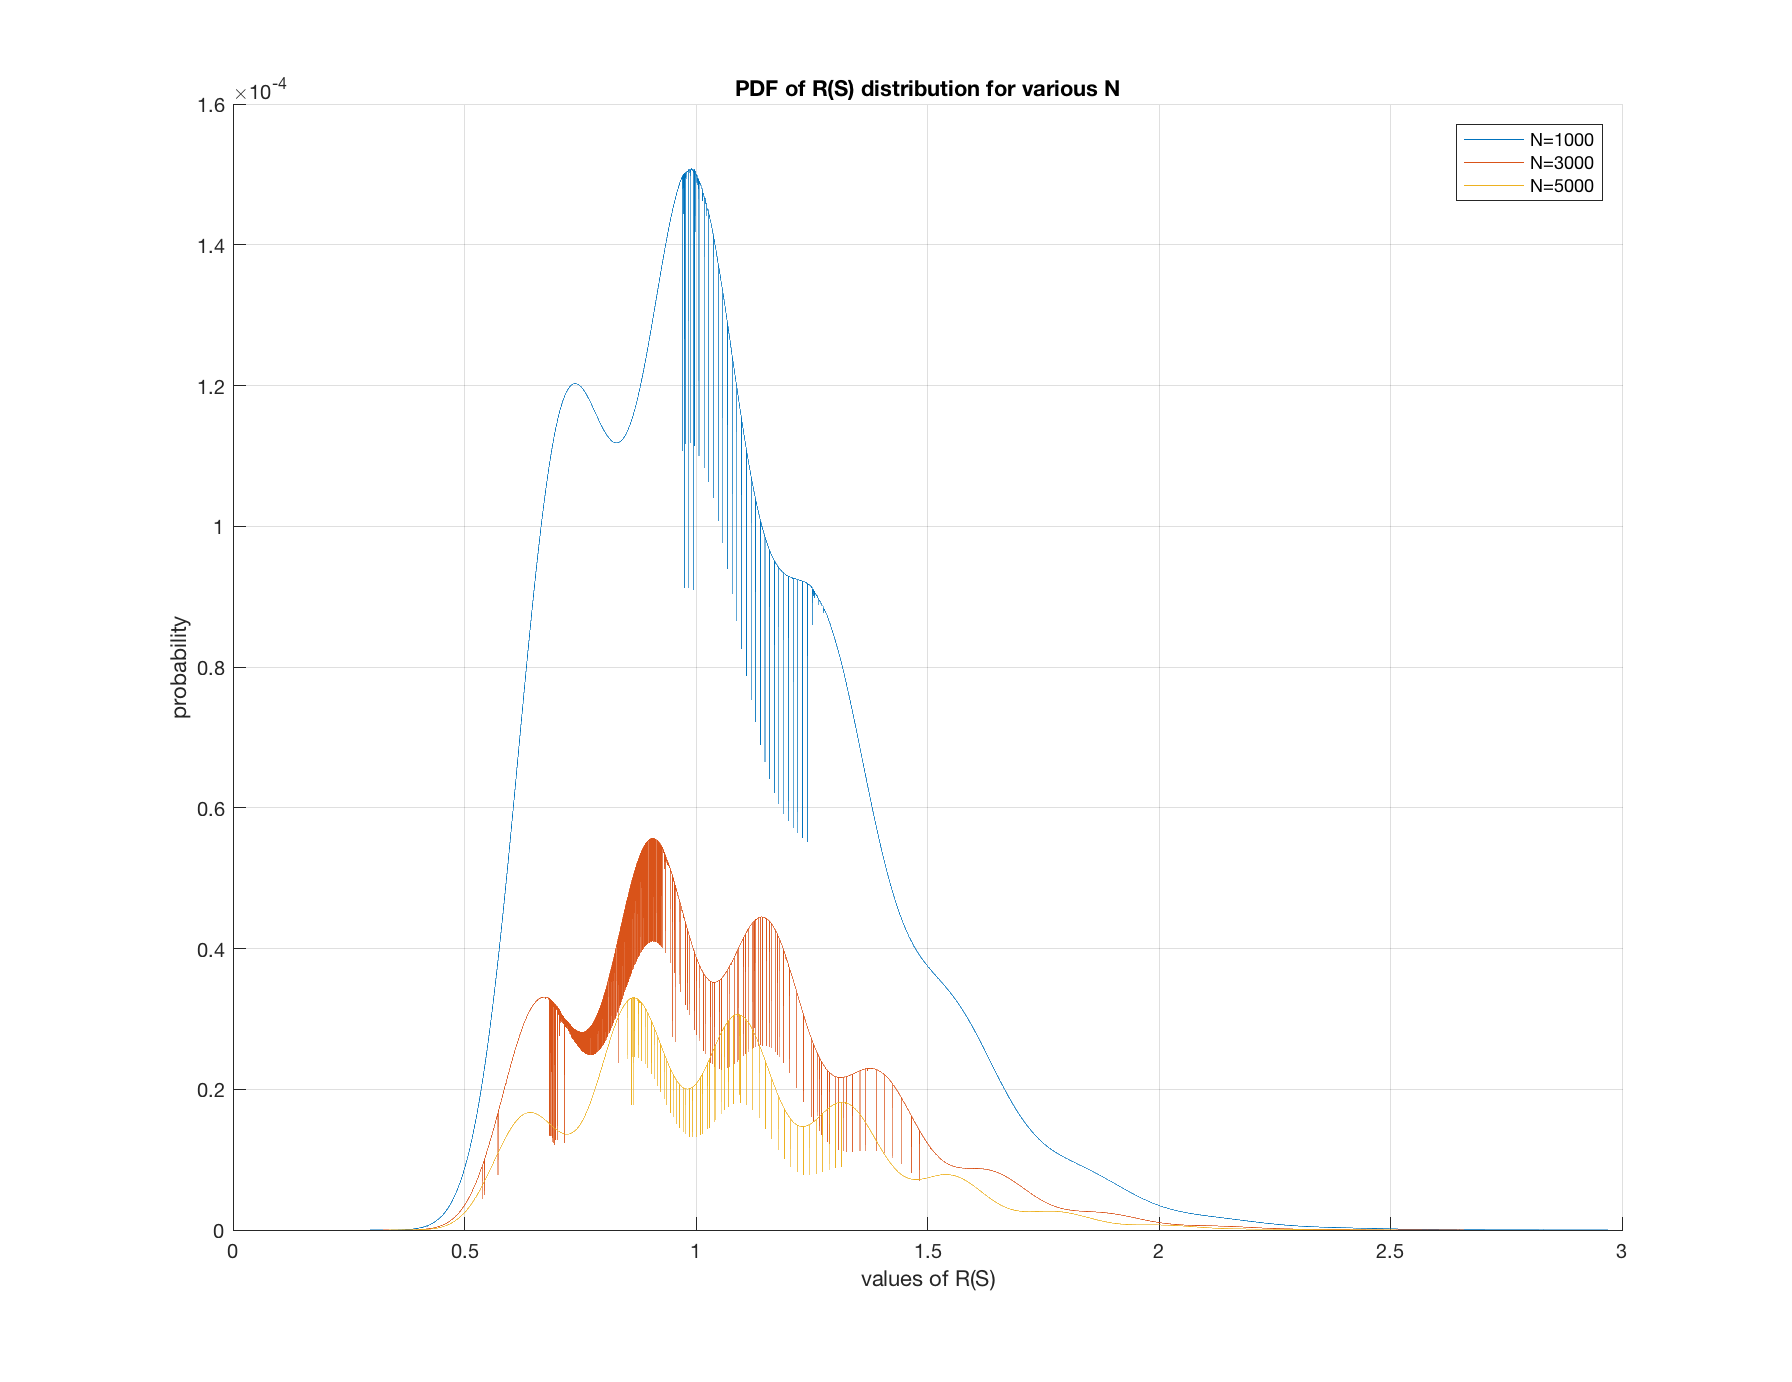
\includegraphics[scale =  0.25]{xyz.png}
 
 The distributions are not exactly bell shaped, but bell shaped enough to keep values of $R(S) \ge 2$ negligibly small. In fact, when loosing the privacy bound by setting  $\lambda = e^2$, the corresponding PDFs  are no longer bell-shaped, but still keep the property of probability mass concentrating below $\mu + 3\sigma$.   The readings and PDFs are given below:
 
  \[
  \begin{matrix}N = 1000 & q = 0.1692 & p(R(S) \ge \lambda) = 0.0037 \\
  N= 3000 & q = 0.1424 & p(R(S) \ge \lambda) = 0.0062  \\
  N=5000 & q = 0.1310 & p(R(S) \ge \lambda) = 0.0074 \end{matrix} 
 \]
 
 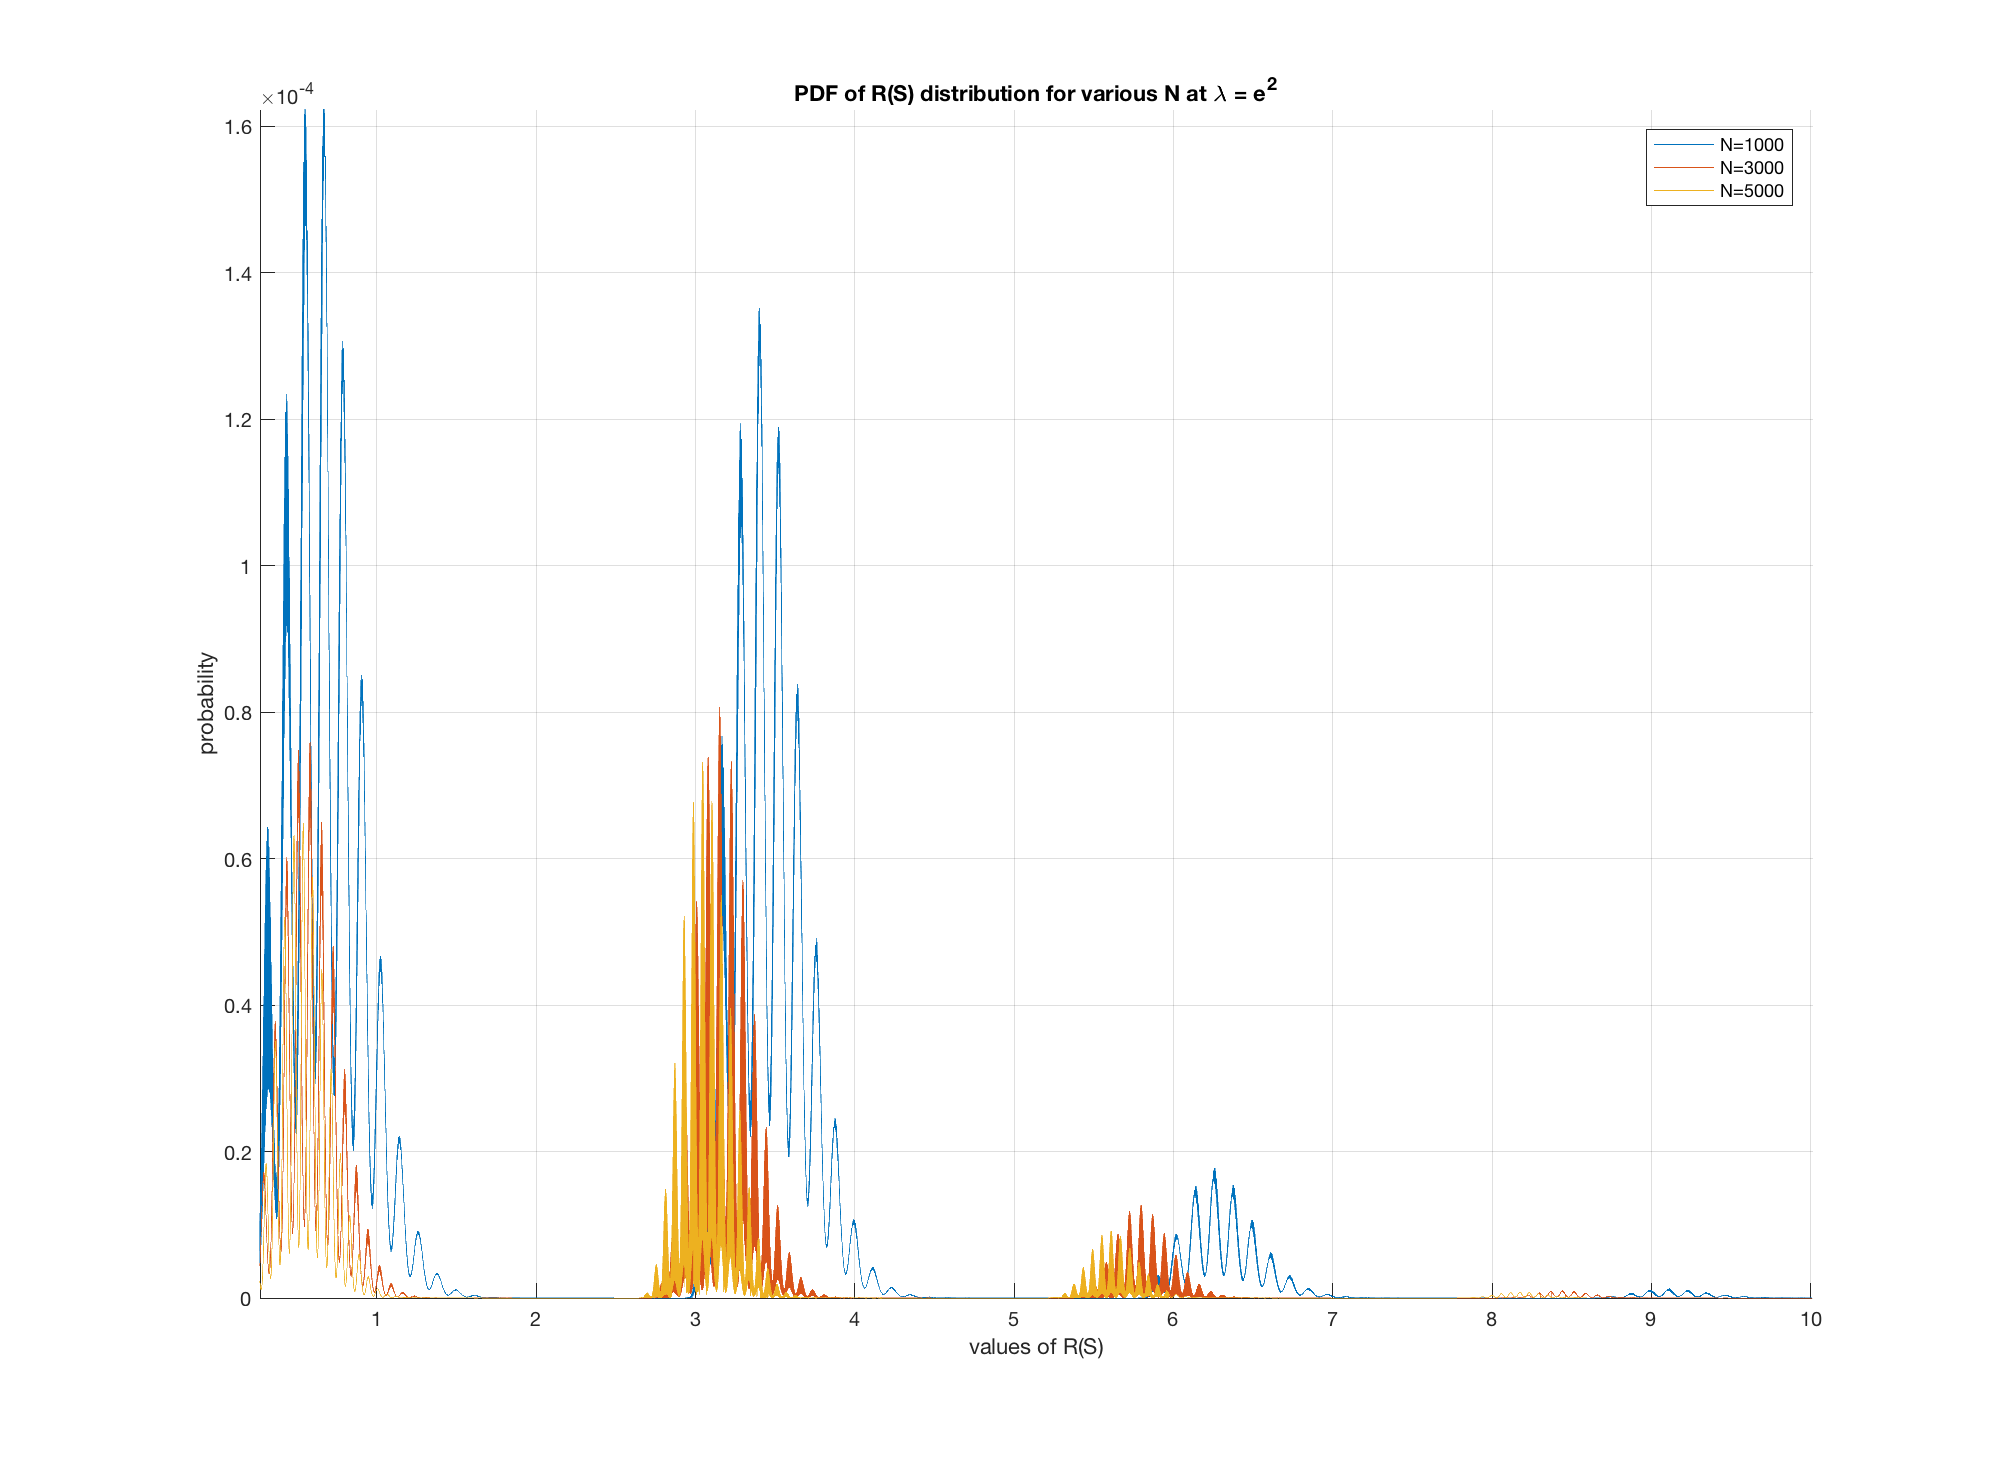
\includegraphics[scale =  0.25]{nPn5.png}
 
 \textbf{Remark}  I believe we can prove concentration phenomena more formally by using Hoeffding's inequality (\url{https://en.wikipedia.org/wiki/Hoeffding%27s_inequality
}) and proving that probabilities are falling exponentially with enough distance from the mean.  Leaving it untouched for now. 

\section{Precision gain}

Suppose that the original collection consists only of indicator bit vectors, each having exactly one set bit, and that the bit in position $j$ is set for $d$ out of the $N$ vectors.
The number $M$ of synthetic vectors (generated by $A_0$) whose $j$-th bit is set has expectation
\[ \EP M = p \cdot d + q \cdot (N-d) \]
Hence, we can estimate $d$ as
\[ \hat{d} = \frac{M-qN}{p-q}. \]
The expectation and standard deviation of the estimate $\hat{d}$ are given by:
\begin{align*}
\EP \hat{d} &= d \\
\sigma( \hat{d}) &= \frac{\sqrt{qpN}}{p-q} = \sqrt{N} \frac{\sqrt{qp}}{p-q}
\end{align*}

How much exactly does the aggregate precision improve with RRT noise reduction?
Consider $\sigma$: the $\sqrt{N}$ component is present regardless of the noise, but the remaining value is highly dependent on $q$.  Below is the  graph of such dependency:

 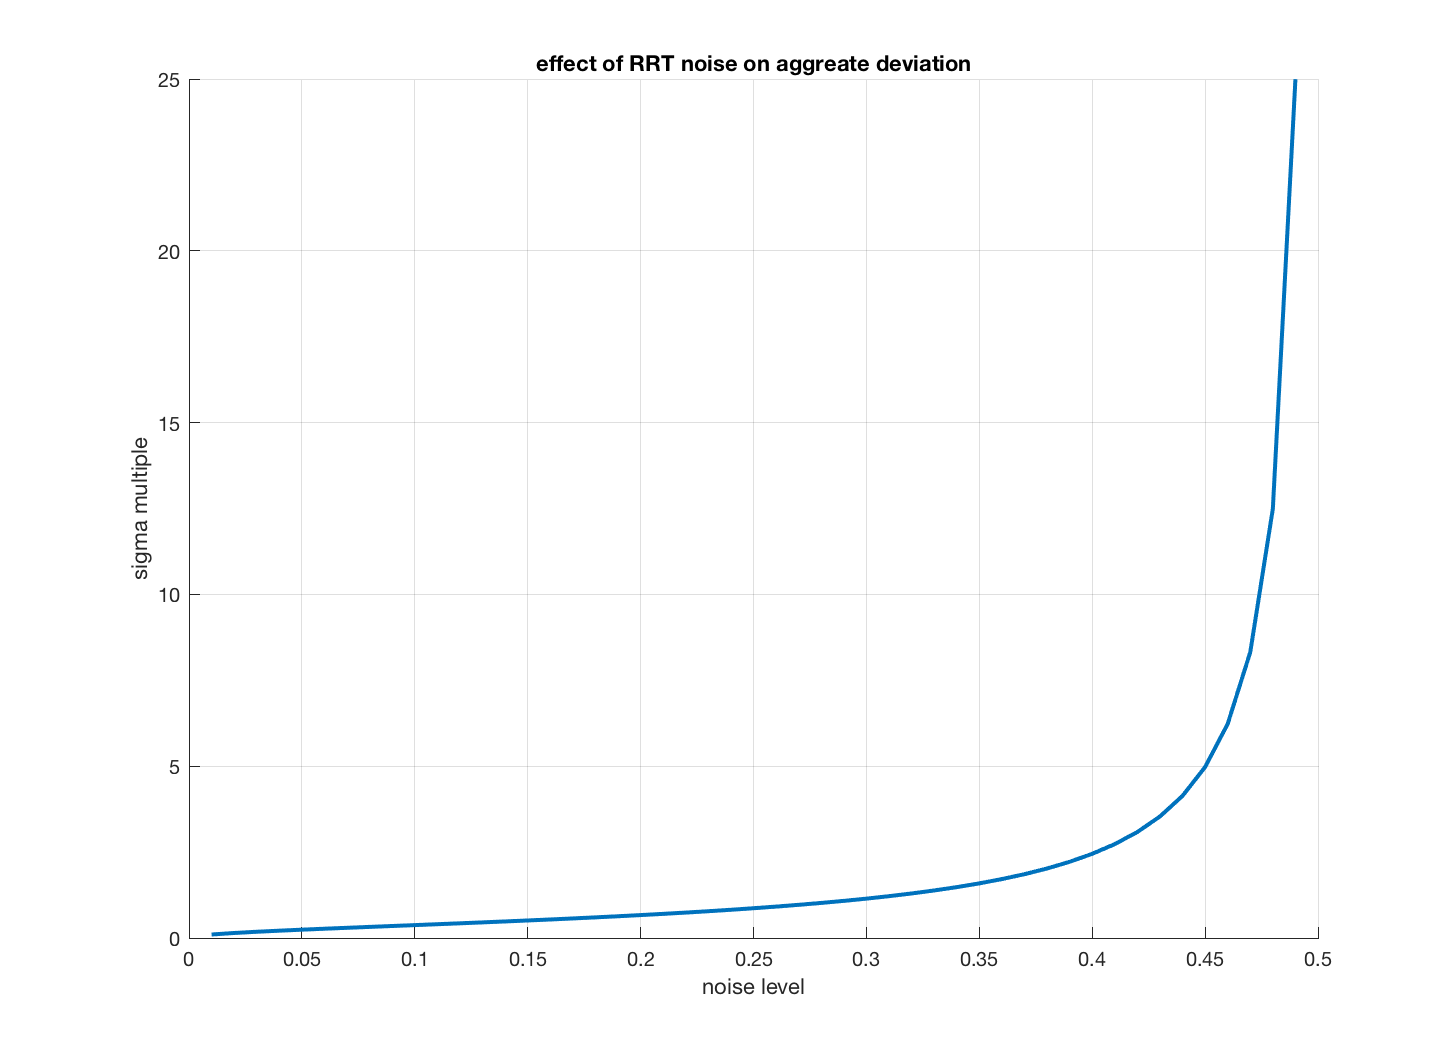
\includegraphics[scale =  0.25]{noise_effect.png}

It actually could be very significant.  Even for relatively short bit vectors of size $L=5$, the required local DP noise is:
 \begin{align}
\left ( \frac{p}{q} \right )^L \le \lambda = e^\epsilon \\
q \ge \frac{1}{1+ \lambda^{\frac{1}{L}}}
\end{align}

Using our example above for $\lambda = 2$, the local DP noise is:
 \begin{align}
q = \frac{1}{1+ \lambda^{\frac{1}{L}}}= 0.465
\end{align}

This noise level results in estimate deviation equal to $\sigma = 7.5 \sqrt{N} $.  However, if we take into account that there are $5000$  records contributing to synthetic collection and employ sufficient privacy, the corresponding noise level is only $q=0.1778$ and deviation becomes $\sigma = 0.6 \sqrt{N} $.  This is $12$ fold increase in precision! 

Consider a far more radical example.  Suppose $L=40$ and $N=10M$.   This actually resembles a typical use case: $40$ bits is a sufficiently long vector to encode user data, while $10M$ users is very achievable given todays massive audiences.  Even if privacy bound is loose ($\lambda=e^2$), the local DP may not provide useful utility.  The required noise for local DP is $q=0.4875$.  The noise that high increases deviation $20$ times!  In practical terms, it means that measured aggregates could deviate $200K$ units in either direction.  This is a very, very bad aggregation quality, unlikely to meet any business goal save the very crude estimates of very large sub-populations.

Contrast that to the precision the sufficient privacy enables.  The required noise is $q=0.351$ which multiples deviation only by $1.6$ (the $12.5$ precision increase again).  And the measurer will be able to estimate with the error not exceeding $15K$.  Which is  sufficient to estimate even 1\% of the population with 10\% error.  Which seems to provide utility good enough for  many practical applications.

\section{Cardinality reduction for partially filled vectors}

Often enough an original vector may only contain a certain number of set bits.  A typical use case is when a user can only report a distinct item from a large set of items (a home page, a word typed, am advertisement click, etc..), in which case only one bit is set in the original vector while the rest are all zeros.   One can verify that if bits are mutually exclusive, and a set bit is required, then an outlier collection construction reduces to the setup below:

\begin{align}
v_1 = \underset{L}{\underbrace{100 \dots 00}} \\
v_2 = \underset{L}{\underbrace{100 \dots 00}} \\
v_3 = \underset{L}{\underbrace{100 \dots 00}} \\
\dots \\
v_{N} =  \underset{L}{\underbrace{010 \dots 00}} 
\end{align}

The original collection has $1$ in the first column and the only legal modification one can make is to switch a bit in the first column to $0$ and set $1$ bit in any other column.  Hence, an outlier could only be different from a vector of the original collection by at most $2$ bits.  Privacy protection wise, this setup is is an equivalent for the $2$ bit zero-valid collection of:
\begin{align}
v_1 = \underset{2}{\underbrace{00}} \\
v_2 = \underset{2}{\underbrace{00}} \\
v_3 = \underset{2}{\underbrace{00}} \\
\dots \\
v_{N} =  \underset{2}{\underbrace{11}} 
\end{align}

Even tough $L$ could be arbitrary long, the amount of noise vectors encoding mutually exclusive categories only need noise enough to protect collections of $2$ but vectors that allow for any bit value in any bit position.

In fact, if can shown that if an original vector is not allowed to have more than $k$ set bits, the amount of sufficient privacy noise to protect such vectors is the same as for collection of arbitrary bit vectors of size $L = 2k$. 

\textbf{Remark}  Intuitively this claim makes sense.  We still may want to show formally that $R(S)$ expression for those setups are equivalent. 


\section{Appendix 1 - expectations and variances for $X_0$ and $X_1$ contributions}

For zero-valued vector contribution $X_0$:
\begin{align}
E(X_0)=  G'(X_0) = \sum_{l=0}^{L} \binom{L}{l} q^lp^{L-l} \left ( \frac{q}{p} \right )^ {L - 2l} = \sum_{l=0}^{L}  \binom{L}{l} \cdot q^{L-l}p^{l} = (p+q)^L = 1 \\
VAR(X_0)=  G''(X_0) - (E(X_0))^2 + E(X_0) = G''(X_0) - 1 + 1 =  G''(X_0) \\
 G''(X_0) = \sum_{l=0}^{L} \binom{L}{l} q^lp^{L-l} \left ( \frac{q}{p} \right )^ {L - 2l} \left [  \left ( \frac{q}{p} \right )^ {L - 2l} - 1 \right ] = \\
  \sum_{l=0}^{L}  \binom{L}{l} \cdot q^{L-l}p^{l}  \left ( \frac{q}{p} \right )^ {L - 2l}  - \sum_{l=0}^{L}  \binom{L}{l} \cdot q^{L-l}p^{l}  =   \sum_{l=0}^{L}  \binom{L}{l}   \frac{q^{2L-3l}}{p^{L-3l}}  - 1 = \\
\sum_{l=0}^{L}  \binom{L}{l}   \frac{q^{3L-3l} p^{3l}}{(pq)^{L}} - 1 =  \frac{1}{(pq)^{L}} \sum_{l=0}^{L}  \binom{L}{l}   (q^3)^{L-l} (p^3)^{l} - 1 = \left ( \frac{p^3 + q^3}{pq} \right )^L - 1
\end{align}

to restate
\begin{align}
E(X_0)=  = 1 \\
VAR(X_0) = \left ( \frac{p^3 + q^3}{pq} \right )^L - 1
\end{align}

In a similar fashion one derives expectation and variance for $X_1$:
\begin{align}
E(X_1)=  =   \left ( \frac{p^3 + q^3}{pq} \right )^L\\
VAR(X_1) = \left ( \frac{p^5 + q^5}{(pq)^2} \right )^{L}  - \left ( \frac{p^3 + q^3}{pq} \right )^{2L} 
\end{align}

\end{document}

